\section{Newton Polynomial Interpolation}

For some interpolation problem (collocation), a polynomial 
$p(x) = c_0 + c_1x + c_2x^2 + \ldots + c_mx^m$
of degree $m$ is required such that the degree $m$ is minimal while meeting collocation conditions.

The data (measurements) are given by indexed pairs $(x_k,y_k)$ with $k=0,1,2,\ldots,n$.

\subsection{Aitken-Neville Recursion Formula}

Group together polynomials of a subset of the measurement into a global polynomial, e.g. for a dataset with three measurements:

\begin{align*}
	p_{0,1,2}(x)=\frac{(x-x_0)p_{1,2}(x) - (x-x_2)p_{0,1}(x)}{(x_2-x_0)}
\end{align*}

\subsection{Newton Basis Polynomials}

The basis polynomials with degree $k=0,1,2,\ldots,n$:

\begin{snugshade*}
	\begin{align*}
		\pi_0(x) & = 1 \\
		\pi_1(x) & = (x-x_0) \\ 
		\pi_2(x) & = (x-x_0)(x-x_1) \\
		\vdots \\
		\pi_n(x) & = (x-x_0)(x-x_1)\ldots(x-x_{n-1})
	\end{align*}
\end{snugshade*}

can be used to form a collocation polynomial using a linear combination 
$p(x)=a_0\pi_0(x) + a_1\pi_1(x) + \ldots + a_m\pi_m(x)$. 
This forms the system of linear equations
\begin{align*}
	y_0 & = a_0 \\
	y_1 & = a_0 + a_1(x_1-x_0) \\
	y_2 & = a_0 + a_1(x_1-x_0) + a_2(x_2-x_0)(x_2-x_1) \\
	\vdots \\
	y_n & = a_0+a_1\pi_1(x_n)+a_2\pi_2(x_n)+\ldots+a_n\pi_n(x_n)
\end{align*}

\emph{Stability}: Since the coefficient $a_k$ is determined by the first $k$ arguments,
we can extend the dataset with new data without altering existing coefficients.

\subsubsection{Divided Differences}

Due to stability, we can write the coefficients as $a_k(x_0,\ldots,x_k)$, only depending on the arguments lower than $k$.
Applying the Aitken-Neville formula, we receive for $k=0,1,\ldots,n$:

\begin{align*}
	y(x_0, x_2, \ldots, x_k)=\frac{y(x_1,x_2,\ldots,x_k) - y(x_0, x_1, \ldots, x_{k-1})}{(x_k - x_0)}
\end{align*}

\makebox[\columnwidth]{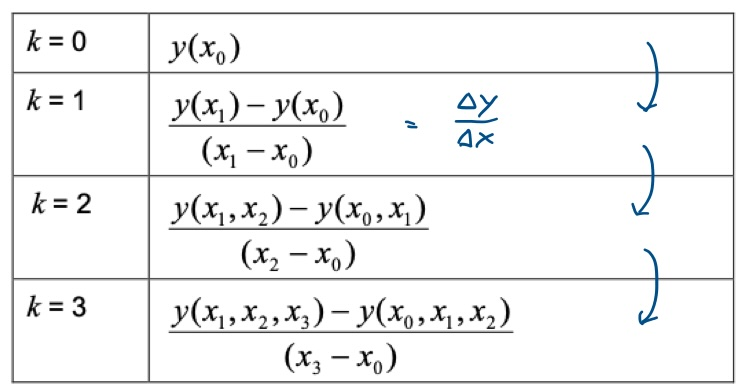
\includegraphics[width=0.6\columnwidth]{images/aitken-neville}}

\makebox[\columnwidth]{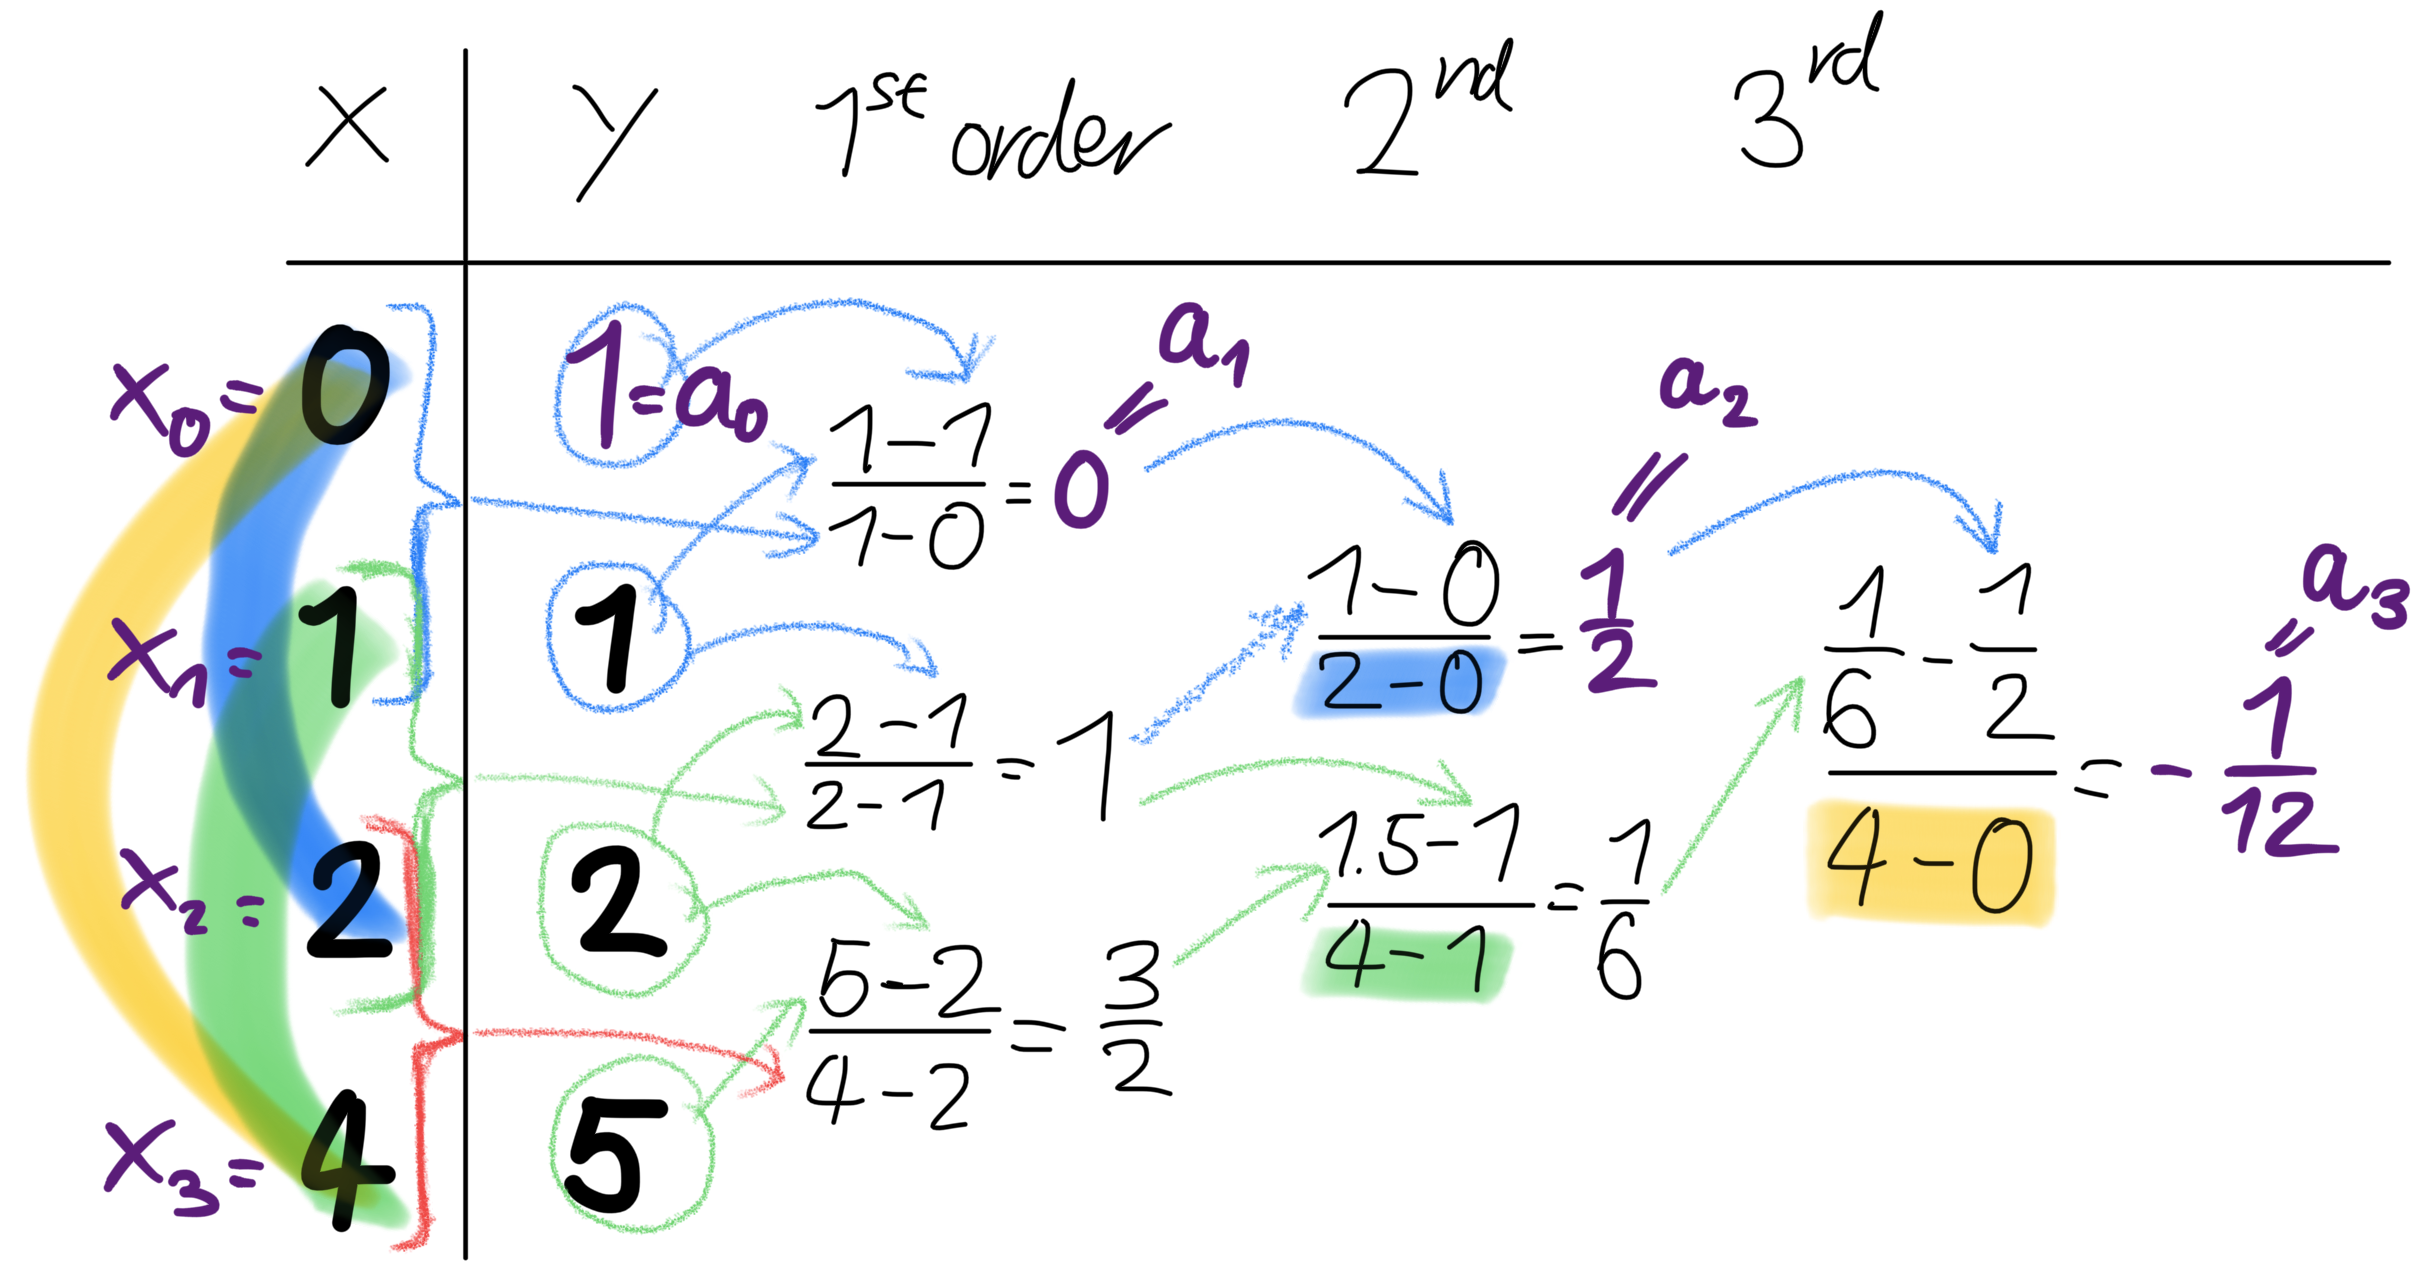
\includegraphics[width=0.6\columnwidth]{images/divided-differences}}
